%The following is a template for including figures:

\begin{figure}[h]
\includegraphics[width=\textwidth]{<file_name>}
\caption{<caption>}
\label{fig:<figure_label>}
\end{figure}


% Figures from the paper will enter thesis in the following order:

% 1. Decay diagrams
\begin{figure}[h]
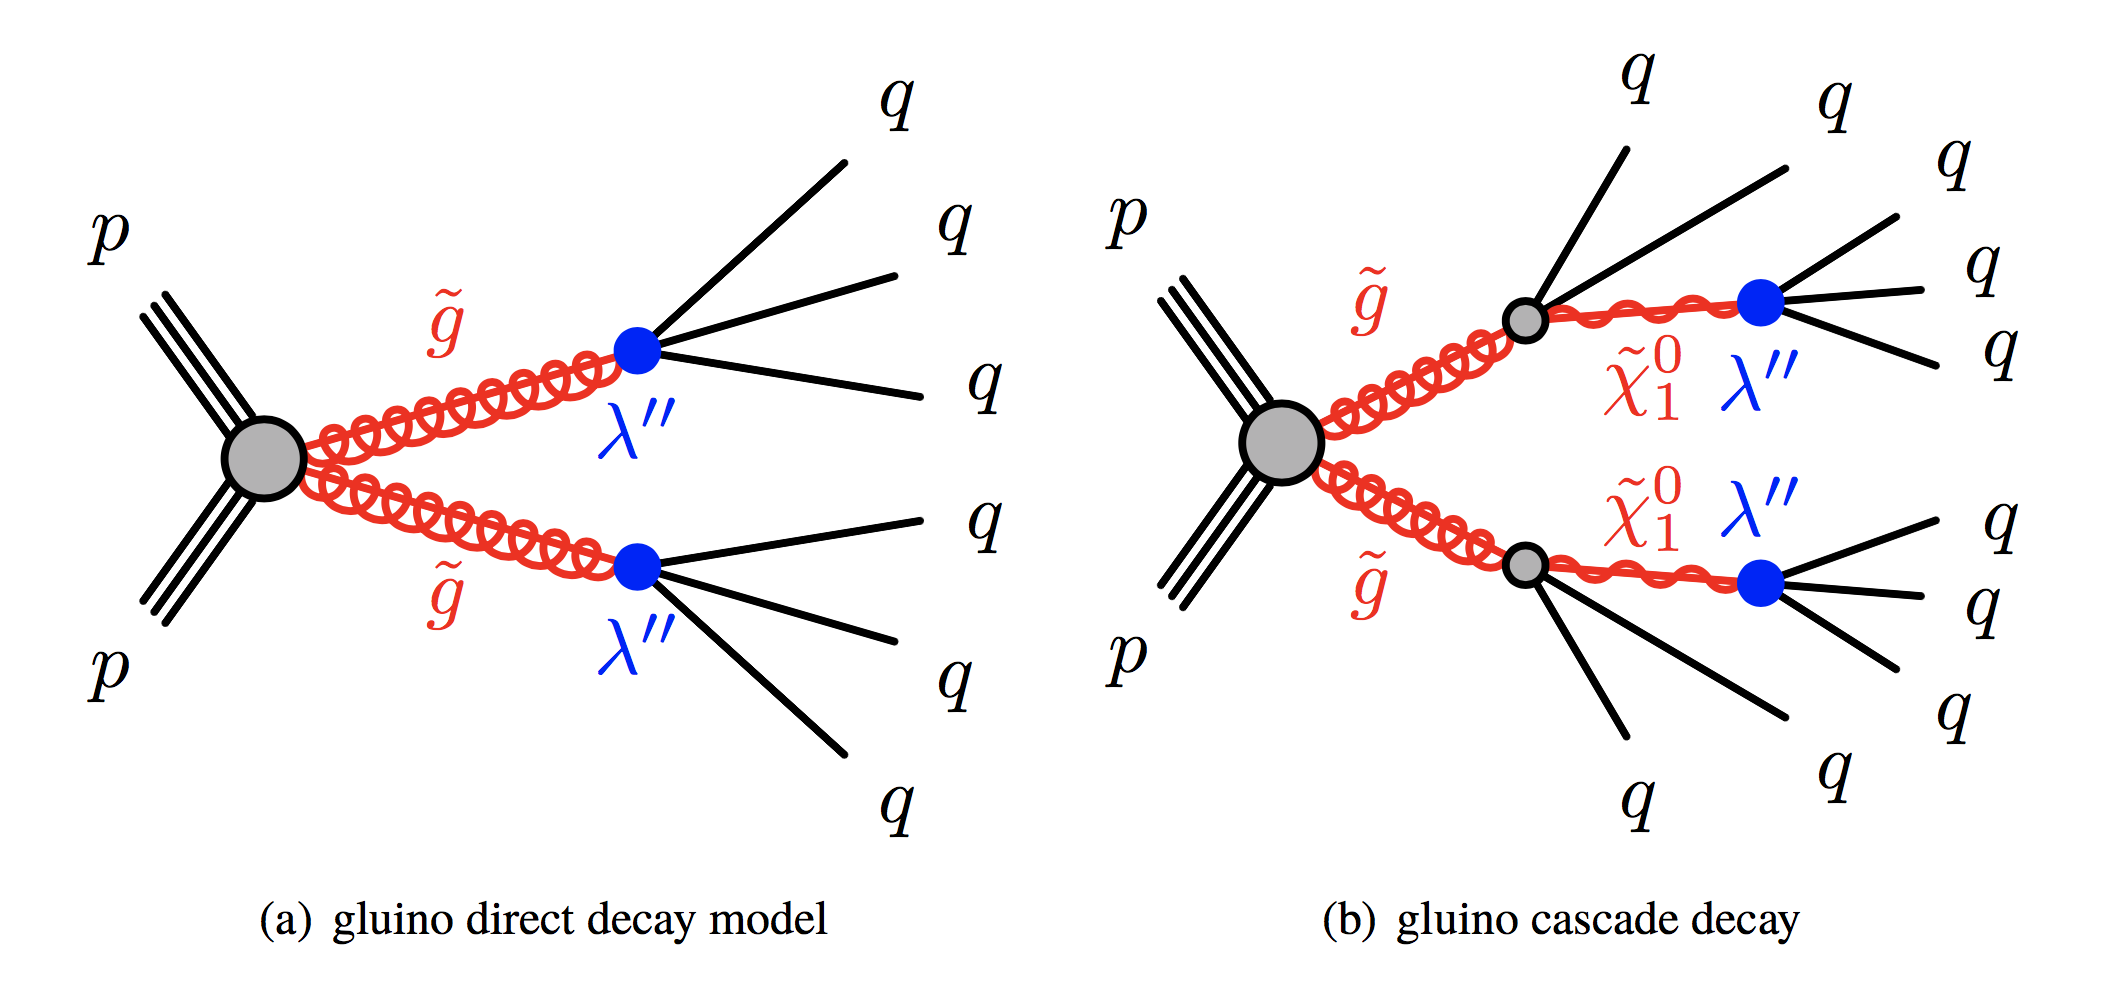
\includegraphics[width=\textwidth]{decay_diagrams_combined}
\caption{Diagrams illustrating the direct and cascade decay modes considered. The blue circles indicate the effective vertices, arising from an off-shell squark decaying to two quarks. At energies far below the squark mass, the contribution to the amplitude from each blue vertex is proportional to $\lambda''$.}
\label{fig:decay_diagrams}
\end{figure}

% 2. MJ / dEta distributions
%used



% 3. Observed MJ distributions, VRs
\begin{figure}[h]
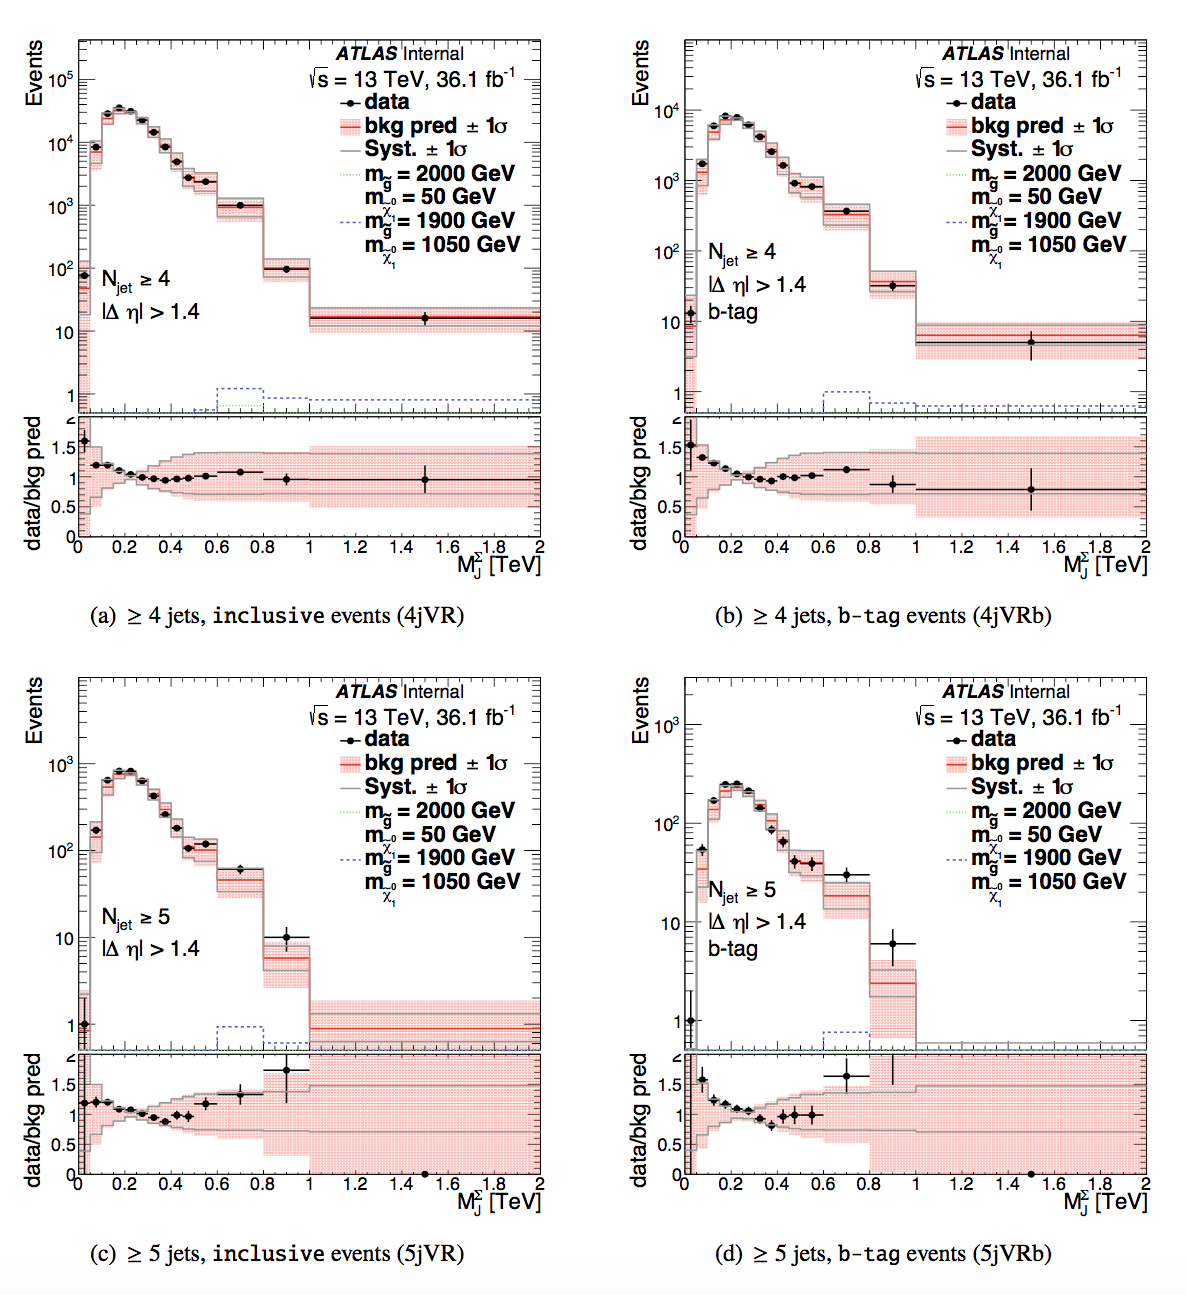
\includegraphics[width=\textwidth]{predicted_and_observed_MJ_VRs}
\caption{}
\label{fig:pred_obs_MJ_VRs}
\end{figure}

% 4. Observed MJ distribtuions, SRs
\begin{figure}[h]
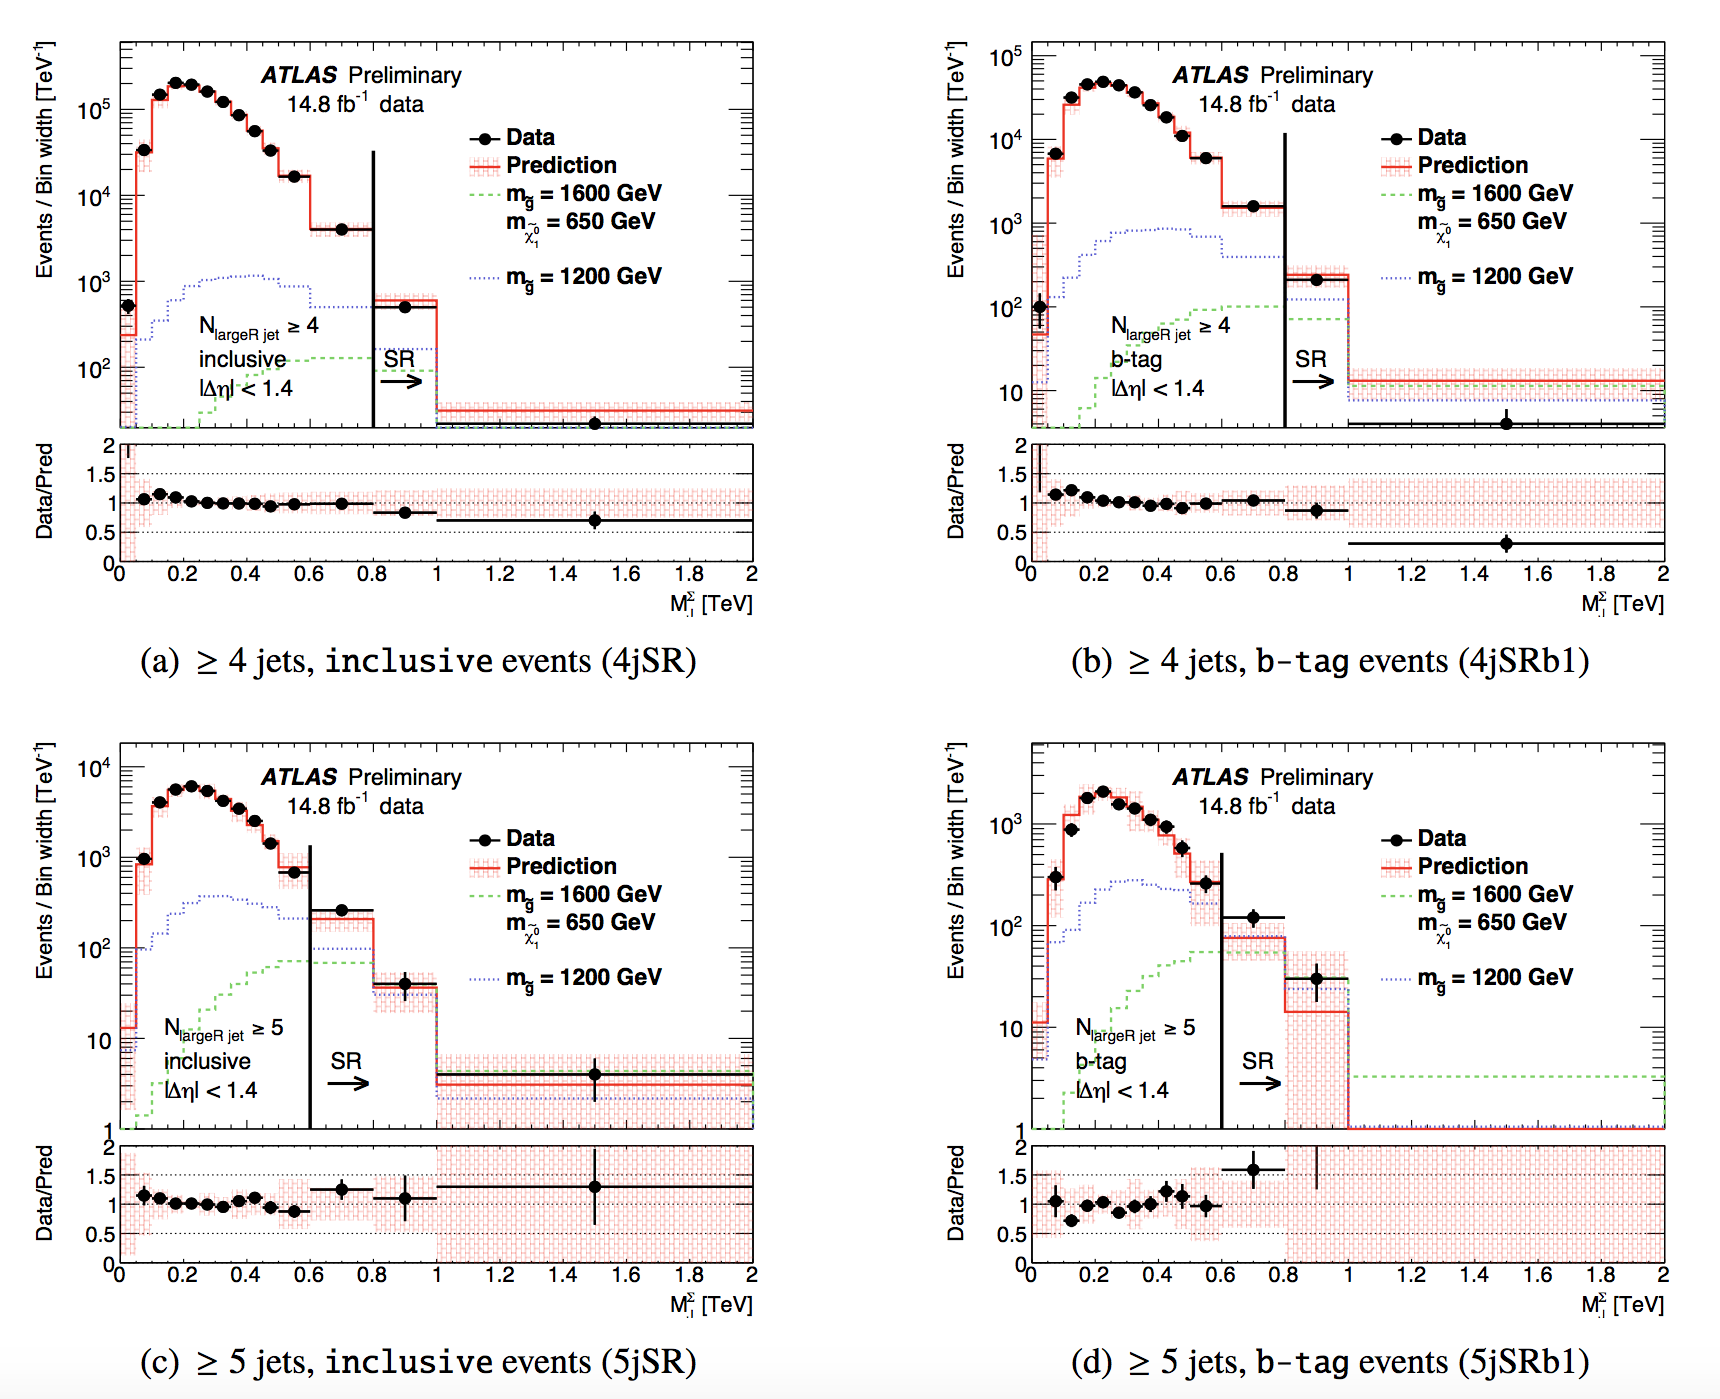
\includegraphics[width=\textwidth]{predicted_and_observed_MJ_SRs}
\caption{}
\label{fig:pred_obs_MJ_SRs}
\end{figure}

% 5. Limit plots
\begin{figure}[h]
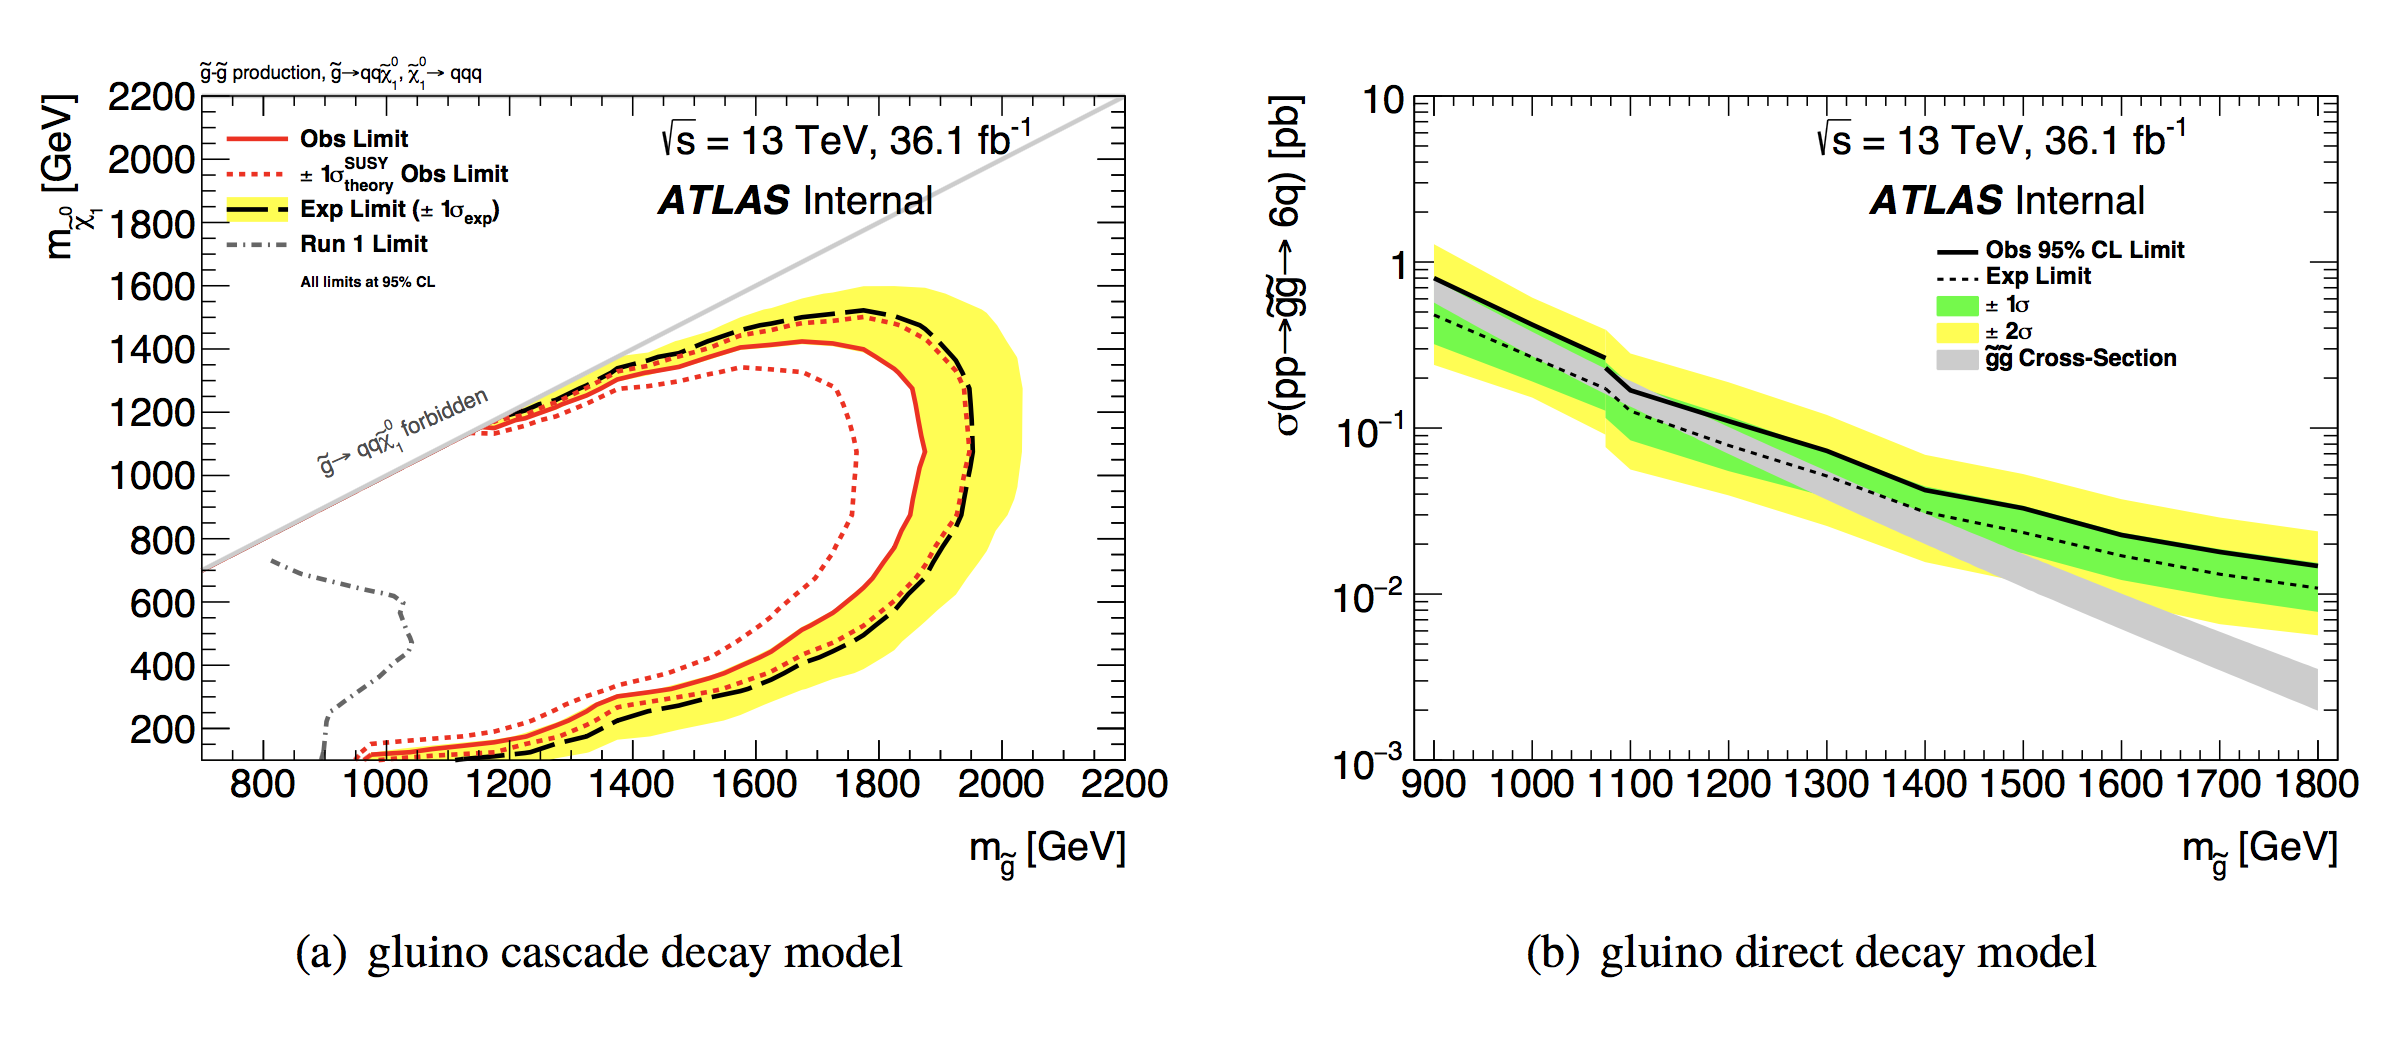
\includegraphics[width=\textwidth]{limit_plots}
\caption{}
\label{fig:limits}
\end{figure}
